\documentclass[a4paper]{article}
\usepackage{libertine}
\usepackage[T1]{fontenc}
\usepackage[utf8]{inputenc}
\usepackage{geometry}
\geometry{%
	left   = 2cm,
	right  = 2cm,
	top    = 2cm,
	bottom = 2cm
}
\usepackage{setspace}
\setstretch{1}
\usepackage{amsmath}
\usepackage{amssymb}
\usepackage[nolist]{acronym}
\usepackage{commath}
\usepackage{verbatim}
\usepackage{booktabs}
\usepackage{listings}
\usepackage{enumitem}
\usepackage{graphicx,color,psfrag}
\usepackage{subfigure}
\usepackage{wrapfig}
\usepackage{svg}
\usepackage{svg-extract}
\usepackage{todonotes}
\usepackage[acronym,nonumberlist,nowarn,style=long]{glossaries}
\usepackage{color}
\usepackage{tikz}
\usepackage{pgf-umlsd}
\usepackage{ifthen}
\usepackage{hyperref}


\newacronym{acr:FPGA}{FPGA}{field programmable gate array}
\newacronym{acr:IP}{IP}{intellectual property}
\newacronym{acr:ILA}{ILA}{integrated logic analyzer}
\newacronym{acr:CNN}{CNN}{convolutional neural network}
\newacronym{acr:DMA}{DMA}{direct memory access}
\newacronym{acr:PS}{PS}{processing system}
\newacronym{acr:PL}{PL}{programmable logic}
\newacronym{acr:BRAM}{BRAM}{block-RAM}

\begin{document}
% This is used to limit the number of authors
% Unfortunatly only working on IEEE
% \bstctlcite{IEEEexample:BSTcontrol}

\begin{titlepage}
	
	\begin{flushright}
		
		% Update this with your team number]
		
		% Update this with your matriculation number, first name, second name
		\Large 
		Yellow Of The Egg\\
		\large
		Lukas Baischer	\\
		Benjamin Kulnik	\\
		Stefan Marschner \\
		add your names \dots \\
		
	\end{flushright}
	
	\vspace{5em}
	
	\begin{center}
		{\Large SoC Design Laboratoy}\\[1em]
		{\large 384.157, Winter Term 2019} \\[5em]

		
		{\Huge MNIST-FPGA\\[.5em]
		\huge Specification}\\[10em]
	\end{center}

\end{titlepage}


\begin{acronym}
	\acro{FPGA}{Field Programmable Gate Array}
	\acro{FIFO}{First In, First Out}
	\acro{CNN}{Convolutional Neural Network}
\end{acronym}
\section{Introduction}


\section{Concept}
\begin{figure}[h]
	\centering
	\includesvg[width=\textwidth]{img/inkscape/NN-concept.svg}
	\caption[Top-Level concept.]{Top-Level concept}
	\label{FIG:concept}
\end{figure}
\todo{Maybe add an additional Input Layer which is responsible to communicate with the DMA and converts the data from 32 bit to 8 bit and sends it to the memory controller}
\noindent
Figure \ref{FIG:concept} shows the Concept of implementing an FPGA-based hardware accelerator for handwritten digit recognition. It shows that the main components of the concepts are a Zedboard in combination with a remote PC or server. The handwritten digit recognition is performed by the Zedboard while the remote PC is used for training the network, for sending the image data to the Zedboard and for receiving the computed results.  The Zedboard includes a Zynq-7000 FPGA and provides various interfaces. \\
The neural network is implemented in the programmable logic part of the Zynq-7000. It is pre-trained using the remote PC, therefore only the inference of the neural network is implemented in hardware. \\
In order to train the network with the same bit resolution as implemented in the hardware, a software counterpart of the hardware is implemented in a PC using python. 
Based on the weights calculated by the python script a bitstream for the hardware is generated. This brings the benefit that for the convolutional layer constant multiplier can be used, since the weights of convolutional layer kernels are constant. For the dense layer it is not possible to implement the weights in a constant multiplier because in a dense layer each connection of a neuron requires a different weight, which would result in a huge amount of required constant multipliers. Therefore the weights for the dense layer have to be stored in a ROM inside the FPGA.   \\


\section{Software}

\subsection{Neural Network Design and Training}
\label{subsec:nntraining}

%\begin{wrapfigure}{r}{0.5\textwidth}
%	\centering
%    \includegraphics[width=0.35\textwidth]{img/nnlayout}
%	\caption{Network Layers}
%	\label{fig:network-layers}
%\end{wrapfigure}

\begin{figure}
	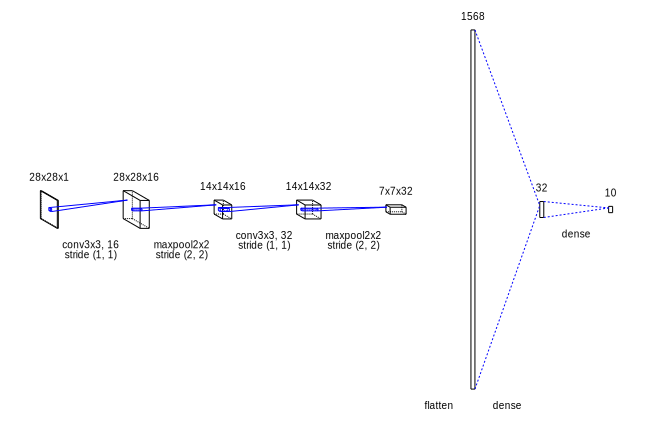
\includegraphics[width=0.8\textwidth]{../../net/images/network}
	\caption{Network overview}
	\label{fig:network-structure}
\end{figure}


The network was implemented in PyTorch \cite{Paszke:2019aa} as well as Tensorflow \cite{MartinAbadi:2015aa}. The backend was later exclusively switched to PyTorch (which is also the most common deep learning framework in Science) due to its better support of qunatization. The layers of the neural network can be seen in Figure~\ref{fig:network-structure}. 
For training of the network the \emph{ADAM} optimization algorithm \cite{Kingma:2014aa} was used to minimize the cross-entropy-loss function which is defined as
\begin{equation}
    J = - y  \log(h) + (1-y)  \log(1-h)
\end{equation}
For controlling the ADAM algorithm the recommended values, listed in Table~\ref{tab:train-params}, by \cite{Kingma:2014aa} was used.
\begin{table}[ht]
	\centering
    \caption{Network Training Parameters}
    \begin{tabular}{cc}
        \toprule
            Parameter & Value \\
        \midrule
            $\alpha$   & $0.001$ \\
            $\beta_1$  & $0.9$   \\
            $\beta_2$  & $0.999$  \\          
        \bottomrule
    \end{tabular}
    \label{tab:train-params}
\end{table}


A useful guide for implementing convolutions can be found in \cite{dumoulin2016guide}. The training 
of the network yielded very high accuracy rates - which is typical for the MNIST dataset, which is for
Machine Learning an easy challenge. Even though the network performance could be improved, e.g. by 
hyperparameter tuning the results were acceptable for our case. The progress of the training in terms
of accuracy and loss can be seen in Figure~\ref{fig:network-train-acc} respectively in Figure~\ref{fig:network-train-loss}.
The final output of the network over the training is evaluated in Figure~\ref{fig:network-test-cm} for real
values and in Figure~\ref{fig:network-test-qcm} for fake quantized values.

\begin{figure}[htbp]
\centering
\begin{subfigure}[t]{0.5\textwidth}
	\includegraphics[width=0.8\textwidth]{../../net/images/training_loss}
	\caption{Training Loss}		
	\label{fig:network-train-loss}
\end{subfigure}%
~
\begin{subfigure}[t]{0.5\textwidth}
	\includegraphics[width=0.8\textwidth]{../../net/images/training_accuracy}
	\caption{Training Accuracy}
	\label{fig:network-train-acc}		
\end{subfigure}
\caption[Network loss and accuracy over the training iterations]{Network loss and accuracy over the training iterations. The blue lines show spikes which occur because of the randomly selected mini batches.}
\label{fig:network-training-graphs}
\end{figure}

\begin{figure}
\centering
\begin{subfigure}[t]{0.5\textwidth}
	\includegraphics[width=0.9\textwidth]{../../net/images/cm}
	\caption{Floating Point}
	\label{fig:network-test-cm}
\end{subfigure}%
~
\begin{subfigure}[t]{0.5\textwidth}
	\includegraphics[width=0.9\textwidth]{../../net/images/qcm}
	\caption{Quantized Values}
	\label{fig:network-test-qcm}
\end{subfigure}
\caption{Confusion matrix for the floating point and quantized version of the netowork.}
\label{fig:network-confusion-matrix}
\end{figure}


\subsection{Quantization}

The network is trained and created using 32bit floating point values in Python. Directly porting this all the weights and biases to the FPGA is due to the limited amount of available resources not feasible. The goal is therefore to reduce the amount of required hardware cells by switching from floating point arithmetic to the less expensive integer arithmetic. Then a floating point value $v$ can be approximately represented as 
\begin{equation}
	v \approx Q \cdot 2 ^{-m}
\end{equation}
where $Q$ and $m$ are integers. In our case all input values of the first layer are guaranteed to lie in the interval $[0,1]$ and all layer weights are known from training. It is therefore possible to precompute the expected range where the output values will be. Depending on this range it is then possible to select a suitable bit width for both $Q$ and $m$.

This is a cost-accuracy trade-off where higher bit widths would improve accuracy as well as increase the amount of hardware resources needed.
In \cite{Wu:2018aa} different strategies of choosing bit widths for $Q$ and $m$ are compared and they observed three main configurations, which are (from simple to advanced):
\begin{enumerate}
	\item Use a $(Q,m)$ configuration for the whole network
	\item Use a $(Q,m)$ configuration for each layer
	\item Use a $(Q,m)$ configuration for each output channel 
\end{enumerate}
In the third configuration the authors could reduce the bit widths the most without sacrificing accuracy this increases the complexity in transferring the weights from layer to layer because the additional shift operations are necessary in order to adjust for the different values of $m$.
In \cite{Wu:2018aa} the authors also deduced from their experiments that the accuracy of the weights can be reduced the most, followed by the activations. By analysing the weights of out network (see Figure~\ref{fig:network-weight-distributions}) a per channel quantization is not necessary, because all weights in a Convolutional Layer are equally distributed among the output channels. Another important property that can be noted is the that the weights do have zero mean and most of the values lie very close to zero. Because of the usage of ReLU layer the situation is different for the activations where unsigned integers can be used, the distributions are shown in Figure~\ref{fig:network-activations-distributions}.

Using the distribution histograms we then defined derived the necessary bitwidths for $Q$ and $m$. In our experiments we were able to reduce them to \SI{8}{\bit}, if we used a single configuration for the whole network and also reducing them down to 4bit if the bitwidth configuration is selected for each layer independently with an accuracy drop from around \SI{98.35}{\percent} to \SI{97.37}{\percent}. The strategy to the select the values for $(Q,m)$ was
\begin{enumerate}
	\item Find the value range of the weights and output activations of each layer
	\item Select suitable $(Q,m)$ values that most activations fall in that range
	\item Calculate the bit widths and exponents of the multiplication operation
	\item Add $\lceil \log_2(n) \rceil$ extra bits to account for the accumulation of $n$ values
	\item Compare the accumulated exponents and with the exponents of the successive layers input exponents. The difference is the amount of shift required
\end{enumerate}
It is noteworthy that the values for $m$ do not need to be stored in the final network, because those are only used to determine the amount of shifts between the layers. Also the values need to be clipped to their maximum and minimum values. The complete configuration of the network is summarized in Table~\ref{tab:quantization-linear-params}.

Ad 4 and 5: The transition from a layer to the next often changes the exponent $m$ and the available bitwidth. To account for this the values need to accordingly shifted. Also the decreased bitwidth needs clipping to maximum available values for the target bitwidth. This directly alters the behaviour of the network which should be accounted for during training, which is done via a saturated version of ReLU, defined as:
\begin{equation}
    \text{ReLU}_{\text{sat}}: ~ f(x;p) = \begin{cases}
		0 	\quad \text{if} \quad x < 0 \\
		p 	\quad \text{if} \quad x > p \\
		x	\quad \text{else}
	\end{cases}
\end{equation}

For our network only linear quantization has been used but also non-linear quantization, e.g. in a $\log_2$ way which is proposed in \cite{Lee:2017aa}. Experiments showed that using this technique even further down to \SI{3}{\bit} weights in our case.
Another optimization technique that could be explored is the systematically removing of weights (connections) of the network and reduce the amount of operations needed to be performed, a process referred to as ''pruning'' \cite{Zhu:2017aa}. This was not explicitly performed but is implicitly done by low bit quantization.

\begin{table}[hbt]
  \centering
  \begin{tabular}{lcccc}
	\toprule
    Network Part 	  & $|Q|$ & $m$ & $\pm$ & $v$ (real value range) \\
	\midrule
    Input 		 	  &  8    & 8  & $+$   & $[0,1]  $ \\
    L1: Weights 	  &  4    & 2  & $\pm$ & $[-2,2] $ \\
    L1: Intermediates & 12    & 10 & $\pm$ & $[-2,2] $ \\
    L1: Accumulated   & 16    & 10 & $\pm$ & 		   \\
    \midrule
    L1 $\to$ L2 	  & \multicolumn{4}{c}{Rshift by $10-2$ and clip values in range $[0,15]$} \\
    \midrule
    L2: Input 		  &  4    & 2  & $+$   & $[-2,2] $ 	   \\
    L2: Weights 	  &  4    & 5  & $\pm$ & $[-0.5,0.5] $ \\
    L2: Intermediates &  8    & 7  & $\pm$ & $[-1,1] $ \\
    L2: Accumulated   & 16    & 7  & $\pm$ &  			   \\
    \midrule
    L2 $\to$ L3 	  & \multicolumn{4}{c}{Rshift by $7-0$ and clip values in range $[0,15]$} \\
    \midrule
    L3: Input 		  &  4    & 0  & $+$   & $[0,15] $     \\
    L3: Weights 	  &  4    & 5  & $\pm$ & $[-0.5,0.5] $ \\
    L3: Intermediates &  8    & 5  & $\pm$ & $[-7.5,7.5] $ \\
    L3: Accumulated   & 19    & 5  & $\pm$ &               \\
    \midrule
    L3 $\to$ L4 	  & \multicolumn{4}{c}{Rshift by $5-0$ and clip values in range $[0,15]$} \\
    \midrule
    L4: Input 		  &  4    & 0  & $+$   & $[0,15] $ \\
    L4: Weights 	  &  4    & 5  & $\pm$ & $[-0.5,0.5] $ \\
    L4: Intermediates &  8    & 5  & $\pm$ & $[-7.5,7.5] $ \\
    L4: Accumulated   & 14    & 5  & $\pm$ & $[0,1] $ \\
    \bottomrule
  \end{tabular}
  \caption[Quantization parameters for the 4bit network]{Quantization parameters for the 4bit network. The intermediate terms are the values after the multiplication operation and the accumulated term denotes values after summing up of weighted inputs including bias in a channel.}
  \label{tab:quantization-linear-params}
\end{table}


%% WEIGHT DISTTRIBUTIONS
\begin{figure}[htbp]
    \centering
    \begin{subfigure}[t]{0.5\textwidth}
        \centering
        \includegraphics[height=1.6in]{../../net/images/hist_cn1_k}
        \caption{Convolutional Layer 1}
    \end{subfigure}%
    ~ 
    \begin{subfigure}[t]{0.5\textwidth}
        \centering
         \includegraphics[height=1.6in]{../../net/images/hist_cn2_k}
        \caption{Convolutional Layer 2}
    \end{subfigure}%
    \\
    \begin{subfigure}[t]{0.5\textwidth}
        \centering
        \includegraphics[height=1.6in]{../../net/images/hist_fc1_w}
        \caption{Fully Connected Layer 1}
    \end{subfigure}%
    ~ 
    \begin{subfigure}[t]{0.5\textwidth}
        \centering
         \includegraphics[height=1.6in]{../../net/images/hist_fc2_w}
        \caption{Fully Connected Layer 2}
    \end{subfigure}
    \caption{Distribution of the network weights for the different layers}
    \label{fig:network-weight-distributions}
\end{figure}


%% ACTIVATIONS DISTTRIBUTIONS
\begin{figure}[htbp]
    \centering
    \begin{subfigure}[t]{0.5\textwidth}
        \centering
        \includegraphics[height=1.6in]{../../net/images/hist_ao1}
        \caption{Convolutional Layer 1}
    \end{subfigure}%
    ~ 
    \begin{subfigure}[t]{0.5\textwidth}
        \centering
         \includegraphics[height=1.6in]{../../net/images/hist_ao2}
        \caption{Convolutional Layer 2}
    \end{subfigure}%
    \\
    \begin{subfigure}[t]{0.5\textwidth}
        \centering
        \includegraphics[height=1.6in]{../../net/images/hist_ao3}
        \caption{Fully Connected Layer 1}
    \end{subfigure}%
    ~ 
    \begin{subfigure}[t]{0.5\textwidth}
        \centering
         \includegraphics[height=1.6in]{../../net/images/hist_ao4}
        \caption{Fully Connected Layer 2}
    \end{subfigure}
    \caption{Distribution of the activations for a randomly selected batch of the input data}
    \label{fig:network-activations-distributions}
\end{figure}


\section{Software}

To ease the usage of the network when it is implemented in the FPGA a suitable user driver software is needed. Here it should be possible to send a single or multiple images to the FPGA and collect the estimated results. 

Also because the major development in Machine Learning is done in Python and the Zedboard is able to run Linux it would be beneficial to control the network via Python and embed it in an existing Machine Learning Framework like Keras \cite{Gulli:2017aa} or Torch \cite{Paszke:2019aa}. Additionally the Zedboard needs additional resources of the FPGA if a graphical user interface should be outputted via the HDMI port. Due to the already sparse available resources the GUI was deactivated and the whole communication was done over Ethernet (or for the initial setup a serial connection). 

\begin{itemize}
	\item Write a low level driver in C to communicate with the FPGA
	\item Provide a Python Interface to the driver
	\item Provide a Web control interface
\end{itemize}


\subsection{FPGA Driver}

The user layer driver software implements an interface between the ARM Top-Level software and the driver for the programmable logic. It is implemented in C. It is supposed to handle the entire communication with the driver so that the hardware is only abstractly visible for the ARM Top-Level software.

For example the ARM top-level software sees the network as a class in python which has a methode\_load\_new\_image data with a numpy array as input and a finish signal as a output. This method should call the user layer driver software which handles the communication between user space and kernel space. In a similar way each IP should be a class in python. 

Requirements of the User Layer Driver Software:
\begin{itemize} 
	\item Communication with the kernel space drivers 
	\item Use python wrapper to communicate with ARM Top-Level software
	\item Easy to use interface from Top-Level 
	\item No knowledge of the hardware should be necessary to use the interface
	\item Data encapsulation to avoid the Top-Level Software from corrupting the memory 
\end{itemize}

\subsection{Python Driver Interface}

\subsection{Web Interface}

The webapp should provide an easy yet good interface to control the network and check its functionality. Because most of the networks software logic is done in python, also the backend of the webapp was done with Python Flask \cite{Pallets:2020aa}. This enabled us the quick interfacing between web components and our python code and also made the communication of multiple threads easier.







\subsection{ARM Top-Level Software}
The ARM top-level software receives the image data from a remote device and sends the results back to this device. Control of the hardware.

\subsubsection{Requirements}
\todo{Add more information and specify the requirements}
Requirements of the ARM Top-Level Software:
\begin{itemize} 
	\item Receive image data
	\item Also use image data set already stored on device
	\item send results to remote PC
	\item Send and receive control signals from remote PC
	\item Send image data to driver user layer and receive results from driver user layer
	\item Send and receive status and control signals to driver user layer
	\item Run at start-up 
\end{itemize}

\subsubsection{Dynamic Updating of the Bitstream}

Optional feature: Update Bitstream file using \texttt{/dev/xdevcfg}.

Update: For newer versions it looks like \texttt{/dev/xdevcfg} doesn't exist anymore. The problem is discussed here \footnote{\url{https://forum.digilentinc.com/topic/18194-dynamically-load-bitstream-on-petalinux/}} and a potential solution can be found here. \footnote{\url{https://github.com/Digilent/zynq-dynamic-tools}}

\subsubsection{Interface to remote PC}
See Section \ref{subsec:InterfaceRemoteZed}.  
\subsubsection{Interface to kernel layer}
Python wrapper are used for the interface between the top level software which is programmed in python and the hardware drivers which are programmed in C. For usability a high level interface to the underlying C wrapper is made. 
This header interface can then be wrapped to multiple target languages using \cite{Swig2020}. In our case this was done for Python.

\subsubsection{File Tree of ARM Top-Level software} \label{SEC:ARM-TOP-SW-FILE-TREE} \todo{Update this section. Do we still use the C code or do we plan to implement everything in python?}
\begin{figure}[h] 
	\centering
	{\includegraphics[scale=0.75]{img/software.pdf}} 
	\caption{File tree for the software}
\end{figure} 
\begin{itemize}
	\item \verb|net_def.h| Contains definitions for networking, e.g. ports used.
	\item \verb|dbg.h| Contains debugging macros for logging and error handling.
	\item \verb|definitions.h| Contains information about the neural network, e.g. the number and type of \ac{CNN} stages, layers in the fully connected network, input size and so on.
	\item \verb|server.{c,h}| Handles the connection with the host software.
	\item \verb|main.c| Contains the \verb|main()| function with the main program loop that transmits and manages data to the hardware and from the host system.
	\item \verb|client.py| Handles the connection with the client software.
\end{itemize}

\subsection{User Layer Driver Software}
The user layer driver software implements an interface between the ARM Top-Level software and the driver for the programmable logic. It is implemented in C. It is supposed to handle the entire communication with the driver so that the hardware is only abstractly visible for the ARM Top-Level software.\\
The ARM top-level software sees the network as a class in python which has methods to load a new image data with a numpy array as input and a finish signal as a output. This method should call the user layer driver software which handles the communication between user space and kernel space. In a similar way each IP should be a class in python. \\
Requirements of the User Layer Driver Software:
\begin{itemize} 
	\item Communication with the kernel space drivers 
	\item Use python wrapper to communicate with ARM Top-Level software
	\item Easy to use interface from Top-Level 
	\item No knowledge of the hardware should be necessary to use the interface
	\item Data encapsulation to avoid the Top-Level Software from corrupting the memory 
\end{itemize}

\subsubsection{File Tree of User Layer Driver Software} \todo{Would be nice if we have something similar as in \ref{SEC:ARM-TOP-SW-FILE-TREE}}



\section{Hardware}
\subsection{Memory Controller}
The task of the memory controller is to provide valid data for the NN-layers. It communicates with the Block-Ram. The memory controller is responsible for ensuring that the next layer has valid data at all times. The second task of the memory controller is to save the data of the previous data in a free memory address in the Block-RAM. 
\todo{Is it better to have the shiftregister, we discussed last time in the memory controller, because in this case the layer don't have to know anything about the data it gets}

\subsubsection{Interfaces}
\begin{itemize}
	\item S\_LAYER: interface to previous layer
\end{itemize}
\begin{tabular}{|l|l|l|l|l|}
	
	signal & direction & type & width & description\\
	
\end{tabular}

\begin{itemize}
	\item M\_LAYER: interface to next layer
\end{itemize}
\begin{tabular}{|l|l|l|l|l|}
	
	signal & direction & type & width & description\\
	
\end{tabular}

\begin{itemize}
	\item BRAM\_PORTA: write interface to BRAM
\end{itemize}
\begin{tabular}{|l|l|l|l|l|}
	
	signal & direction & type & width & description\\
	
\end{tabular}

\begin{itemize}
	\item BRAM\_PORTB: read interface to BRAM
\end{itemize}
\begin{tabular}{|l|l|l|l|l|}
	
	signal & direction & type & width & description\\
	
\end{tabular}

\subsubsection{Parameter}
\begin{itemize}
	\item PREVIOUS\_LAYER\_TYPE boolean: {TRUE: conv2d, FALSE: dense} % maybe some additional -> integer type
	\item PREVIOUS\_LAYER\_WIDTH integer: {Row length of input matrix} \todo{use extra parameter for dense or simply use width or heigth, discuss!}
	\item PREVIOUS\_LAYER\_HEIGTH integer: {Collum length of input matrix}
	\item PREVIOUS\_LAYER\_CHANNEL integer: {Row length of input matrix}
	\item NEXT\_LAYER\_TYPE boolean: {TRUE: conv2d, FALSE: dense} % maybe some additional -> integer type
	\item NEXT\_LAYER\_WIDTH integer: {Row length of input matrix} \todo{use extra parameter for dense or simply use width or heigth, discuss!}
	\item NEXT\_LAYER\_HEIGTH integer: {Collum length of input matrix}
	\item NEXT\_LAYER\_CHANNEL integer: {Row length of input matrix}
\end{itemize}
\subsection{conv2d}

\begin{figure}[h]
	\centering
	\includesvg[width=0.7\textwidth]{img/inkscape/conv2d.svg}
	\caption[Conv2d block diagram.]{Conv2d block diagram. For each output channel a conv\_channel module is used. $k$ indicates the number of output channels.}
	\label{FIG:conv2d}
\end{figure}
Figure \ref{FIG:conv2d} shows the block diagram of a conv2d module. It uses $k$ conv\_channel modules to realise $k$ output channels. 
All conv\_channel modules get the same input vector $X_{c_i}$ which consists of $n \cdot 3 \times 1$ vector, in which $n$ is the number of input channels.  
\subsubsection{Interface}
\todo{define input output interface}

\subsubsection{Parameter}
\begin{itemize}
 	\item INPUT\_CHANNEL\_NUMBER : integer
 	\item OUTPUT\_CHANNEL\_NUMBER : integer
 	\item MATRIX\_WIDTH: integer
 	\item MATRIX\_HEIGTH: integer
\end{itemize}
\subsection{conv\_channel}

\begin{figure}[h]
	\centering
	\includesvg[width=0.7\textwidth]{img/inkscape/conv-channel.svg}
	\caption[conv\_channel block diagram.]{conv\_channel block diagram. For each input channel a kernel\_3x3 module is used. $n$ indicates the number of input channels.}
	\label{FIG:conv-channel}
\end{figure}
Figure \ref{FIG:conv-channel} shows the block diagram of a conv\_channel module. It uses $n$ kernel\_3x3 modules to realise $n$ input channels. 
All kernel\_3x3 modules get a different input vector $X_{c_{i1}}$ to $X_{c_{in}}$ which are $3 \times 3$ input matrices.   
\subsubsection{Interface}
\todo{define input output interface}

\subsubsection{Parameter}
\begin{itemize}
 	\item INPUT\_CHANNEL\_NUMBER : integer
 	\item OUTPUT\_CHANNEL\_NUMBER : integer
 	\item MATRIX\_WIDTH: integer
 	\item MATRIX\_HEIGTH: integer
\end{itemize}
\subsection{kernel-3x3}
This modules performs a multiplication of 9 values of length BIT\_WIDTH\_IN with their respective weights which are defined in an
array that can be set with a generic. The multiplication results are then added up, after which a ReLu step is performed where outputs
above 255 are clipped to 255 and outputs below 0 are clipped to 0.
\subsubsection{Interface}
\begin{itemize}
	\item Input interface, a vector of 9 values of length BIT\_WIDTH\_IN.
	\item Output interface, same as conv\_channel.
\end{itemize}
\subsubsection{Parameter}
\begin{itemize}
	\item BIT\_WIDTH\_IN: integer
	\item BIT\_WIDTH\_OUT: integer
	\item WEIGHT: array of 9 integers
	\item WEIGHT\_WIDTH: integer
\end{itemize}
\subsection{NN}

\subsubsection{Operation}
\begin{figure}[h]
	\centering
	\includegraphics[width=1\textwidth]{img/dense.pdf}
	\caption{Diagram of the combined, fully connected NN.}
	\label{FIG:nn}
\end{figure}

The fully-connected neural network is shown in figure \ref{FIG:nn}. It consists of two dense layer instances controlled by a state machine. The output of layer 1 is fed directly into the layer 2. The output of layer 2 are 10 values which represent the confidence that the input image showed a specific number. 

The Serializer module is connected to the previous pooling layer. The $m=32$ output channels need to be converted into a stream of single values of length VECTOR\_WIDTH. For this, the previous pooling layer is stalled by keeping the ready signal low while a vector of $m$ values is serialized.

\subsubsection{Interface}
\begin{itemize}
	\item Input interface, a stream of values of length VECTOR\_WIDTH
	\item Output interface, a vector of 10 values of length VECTOR\_WIDTH
\end{itemize}
\subsubsection{Parameter}
\begin{itemize}
	\item VECTOR\_WIDTH: integer
	\item INPUT\_COUNT: integer
	\item OUTPUT\_COUNT: integer
\end{itemize}
\input{dense-hw.tex}



\section*{Appendix}
\subsection*{Network Operations}
\subsubsection*{Convolutional Operations}

The output of an convolutional layer is defined by
\begin{equation}
   z(i,j) = (f*g)(i,j) = \sum_{m=-\infty}^{\infty} \sum_{n=-\infty}^{\infty} f(m,n) g(m-i,n-j)
\end{equation}


\subsubsection*{Fully Connected Layer}

The output of an fully connected layer is defined by
\begin{equation}
	z = xW + b
\end{equation}
where $x \in \mathbb{R}^{b,m}$,  $W \in \mathbb{R}^{m,n}$ and $b \in \mathbb{R}^{n}$. 

\subsubsection*{Rectified Linear Unit (ReLU)}

\begin{equation}
	f(x) = \begin{cases}
		x \quad \text{if} \quad x > 0 \\
		0 \quad \text{else}
	\end{cases}
\end{equation}


\subsubsection*{Softmax}

\subsection*{Matrix Calculus}

The chain rule for a vectors is similar to the chain rule for scalars. Except the order is important. For $\mathbf{z} = f(\mathbf{y})$ and $\mathbf{y} = g(\mathbf{x}) $ the chain rule is:
\begin{equation}
    \frac{\partial \mathbf{z}}{\partial \mathbf{x}} = \frac{\partial \mathbf{y}}{\partial \mathbf{x}}     \frac{\partial \mathbf{z}}{\partial \mathbf{y}}
\end{equation}




\begin{table}[h]
    \centering
    \begin{tabular}{cc}
        \toprule
            $y$ & $\frac{\partial}{\partial x} y$ \\
        \midrule
            $Ax$     & $A^T$ \\
            $x^T A$  & $A$   \\
            $x^T x$  & $2x$  \\  
            $x^T Ax$ & $Ax + A^Tx$  \\          
        \bottomrule
    \end{tabular}
    \caption{Useful derivatives equations}
\end{table}
\subsection*{Source Code}

All the source code is licensed under the \emph{MIT} Licence and can be found on Github.
\url{https://github.com/marbleton/FPGA\_MNIST}
\todo{Add cite to github using Zenodo (must be done by Anton)}
\input{other}

\bibliographystyle{apalike}
\bibliography{bibhelper,references}

\end{document}